\documentclass{article}

\title{Informe de Laboratorio}

%%%%%%%%%%%%%%%%%%%%%%%%%%%%%%%%%%%%%%%%%%%%%%%%%%%%%%%%%%%%%%%%%%%%%%%%%%%%
%%%%%%%%%%%%%%%%%%%%%%%%%%%%%%%%%%%%%%%%%%%%%%%%%%%%%%%%%%%%%%%%%%%%%%%%%%%%
\newcommand{\itemEmail}{vsullaq@unsa.edu.pe}
\newcommand{\itemStudent}{VLADIMIR ARTURO SULLA QUISPE}
\newcommand{\itemTeacher}{CARLO JOSE LUIS CORRALES DELGADO}
\newcommand{\itemGitHubURL}{https://github.com/Vladimir2003-debug/PW2-LAB07.git}
\newcommand{\itemCourse}{PROGRAMACION WEB 2}
\newcommand{\itemCourseCode}{20231001}
\newcommand{\itemSemester}{III}
\newcommand{\itemUniversity}{Universidad Nacional de San Agustín de Arequipa}
\newcommand{\itemFaculty}{Facultad de Ingeniería de Producción y Servicios}
\newcommand{\itemDepartment}{Departamento Académico de Ingeniería de Sistemas e Informática}
\newcommand{\itemSchool}{Escuela Profesional de Ingeniería de Sistemas}
\newcommand{\itemAcademic}{2023 - A}
\newcommand{\itemPracticeNumber}{07}
\newcommand{\itemTheme}{Relaciones de uno a muchos, muchos a muchos y impresion de pdf y emails}
\newcommand{\itemFlip}{https://flip.com/5f1a56f8}
\newcommand{\itemInput}{08/07/2023}
\newcommand{\itemOutput}{08/07/2023}
%%%%%%%%%%%%%%%%%%%%%%%%%%%%%%%%%%%%%%%%%%%%%%%%%%%%%%%%%%%%%%%%%%%%%%%%%%%%
%%%%%%%%%%%%%%%%%%%%%%%%%%%%%%%%%%%%%%%%%%%%%%%%%%%%%%%%%%%%%%%%%%%%%%%%%%%%

% STYLE CODE
\usepackage{listings}
\usepackage{xcolor}

\definecolor{codegreen}{rgb}{0,0.6,0}
\definecolor{codegray}{rgb}{30, 82, 255}
\definecolor{codepurple}{rgb}{0.58,0,0.82}
\definecolor{backcolour}{rgb}{0.95,0.95,0.92}

\lstdefinestyle{mystyle}{
    backgroundcolor=\color{backcolour},   
    commentstyle=\color{codegreen},
    keywordstyle=\color{magenta},
    numberstyle=\tiny\color{codegray},
    stringstyle=\color{codepurple},
    basicstyle=\ttfamily\footnotesize,
    breakatwhitespace=false,         
    breaklines=true,                 
    captionpos=b,                    
    keepspaces=true,                 
    %numbers=left,                    
    numbersep=5pt,                  
    showspaces=false,                
    showstringspaces=false,
    showtabs=false,                  
    tabsize=2
}
\lstdefinestyle{ascii-tree}{
    literate={├}{|}1 {─}{--}1 {└}{+}1 
}
\lstset{style=mystyle}
\lstdefinestyle{ascii-tree}{
    literate={├}{|}1 {─}{--}1 {└}{+}1 
  }
% COLORS

%Paquetes 
\usepackage{graphicx} % Required for inserting images
\usepackage{array}
\usepackage{multirow}
\usepackage[top=3cm, bottom=3cm, outer=3cm, inner=3cm]{geometry}

\setlength{\headheight}{30pt}
\usepackage{colortbl}
\graphicspath{ {images/} }
\usepackage{listings}


\lstset{basicstyle=\ttfamily,
  showstringspaces=false,
  commentstyle=\color{red},
  keywordstyle=\color{blue}
}
\usepackage[utf8]{inputenc}
\usepackage[hidelinks]{hyperref}
\usepackage{blindtext}
\usepackage{titlesec}

\usepackage{fancyhdr}
\pagestyle{fancy}
\fancyhf{}
\setlength{\headheight}{30pt}
\renewcommand{\headrulewidth}{1pt}
\renewcommand{\footrulewidth}{1pt}
\fancyhead[L]{\raisebox{-0.2\height}{
\includegraphics[width=3cm]{img/logo_episunsa.png}}}
\fancyhead[C]{\fontsize{7}{7}\selectfont	\itemUniversity \\ \itemFaculty \\ \itemDepartment \\ \itemSchool \\ \textbf{\itemCourse}}
\fancyhead[R]{\raisebox{-0.2\height}{
\includegraphics[width=1.2cm]{img/logo_abet}}}
\fancyfoot[L]{\itemEmail }
\fancyfoot[C]{\itemCourse}
\fancyfoot[R]{Página \thepage}

% BIBLIOGRAFIA

\usepackage{biblatex} %Imports biblatex package
\addbibresource{bibliografy/references.bib} %Import the bibliography file

\begin{document}

\vspace*{30px}

\begin{center}	
		\fontsize{17}{17} \textbf{ Informe de Laboratorio \itemPracticeNumber}
\end{center}
 
\renewcommand{\arraystretch}{1.5}

\begin{tabular}{ |m{3cm}|m{2cm}|m{3cm}|m{1.2cm}|m{2.5cm}|m{1cm}| }
    \hline
    
    \multicolumn{6}{|c|}{\cellcolor{red}\textbf{INFORMACIÓN BÁSICA}} \\
    \hline
    \textbf{ASIGNATURA:} & \multicolumn{5}{|l|}{ \itemCourse} \\
    \hline
    \textbf{TITULO DE LA PRÁCTICA:} & \multicolumn{5}{|l|}{\itemTheme} \\
    \hline     
    \textbf{NÚMERO DE PRÁCTICA:} & \itemPracticeNumber & \textbf{AÑO LECTIVO:} & 2023-A & \textbf{NRO. SEMESTRE:} & \itemSemester\\
    \hline     
    \textbf{FECHA DE PRESENTACIÓN: } & \itemInput & \textbf{HORA DE PRESENTACIÓN:} & \multicolumn{3}{|l|}{ \itemOutput } \\
    \hline     
    \multicolumn{4}{|l|}{\textbf{INTEGRANTE (s):}
    - \itemStudent 
    } &  \textbf{NOTA (0-20)} & \\
    \hline
    \multicolumn{6}{|l|}{\textbf{GITHUB :} \url{\itemGitHubURL}} \\
    \hline
    \multicolumn{6}{|l|}{\textbf{FLIP :} \url{\itemFlip}} \\
    \hline
    \multicolumn{6}{|l|}{\textbf{DOCENTE(s): }
    - \itemTeacher 
    } \\
    \hline     
\end{tabular}

\tableofcontents

\section{TAREA}

Reproducir las actividades de los videos donde trabajamos:

\begin{enumerate}
    \item Relación de uno a muchos
    \item Relación muchos a muchos
    \item Impresión de pdfs 
    \item Envio de emails
    \item Crear su video Flipgrid:
\end{enumerate}



\end{itemize}

\section{MATERIALES USADOS}

\begin{itemize}
    \item Sitema Operativo Ubuntu,Windows 10
    \item Django 4.2.2
    \item Python 3.10.6
    \item pip 22.0.2 
    \item git version 2.34.1
    \item virtualenv 20.13.0
    \item postfix software
\end{itemize}

\section{RESOLUCION}
\subsection{ONE TO MANY RELATIONS}
Con el modelo incial que contiene Simple,DateExample y NullExample añadimos Languaje y Framework
Luego procedemos a hacer lo siguiente en la shell de python:

\begin{lstlisting}[caption=Shell de Python]
(env) PS C:\Users\vladimir\eclipse-workspace\PW2 Lab07\model_examples> python .\manage.py shell
Python 3.10.4 (tags/v3.10.4:9d38120, Mar 23 2022, 23:13:41) [MSC v.1929 64 bit (AMD64)] on win32
Type "help", "copyright", "credits" or "license" for more information.
(InteractiveConsole)
>>> from apps.examples.models import Language,Framework 
>>> python = Language(name='Python') 
>>> python.save()
>>> django = Framework(name='Django') 
>>> flask = Framework(name='Flask') 
>>> python          
<Language: Language object (1)>
>>> django.language = python
>>> flask.language = python
>>> bottle = Framework(name='Bottle', language=python) 
>>> django.save()
>>> flask.save()
>>> bottle.save()
>>> java = Language(name='Java')    
>>> spring = Framework(name='Spring' ,language = java)   
>>> java.save()
>>> spring.save()

\end{lstlisting}
En en codigo anterior vemos como crear varios objeto lenguage, para posteriormente crear objetos framework que al momento de crearlos en la parte de language tenemos que seleccionar uno de los lenguajes ya creados Esto se ve en la imagen 1

\begin{figure}[h]
    \centering
    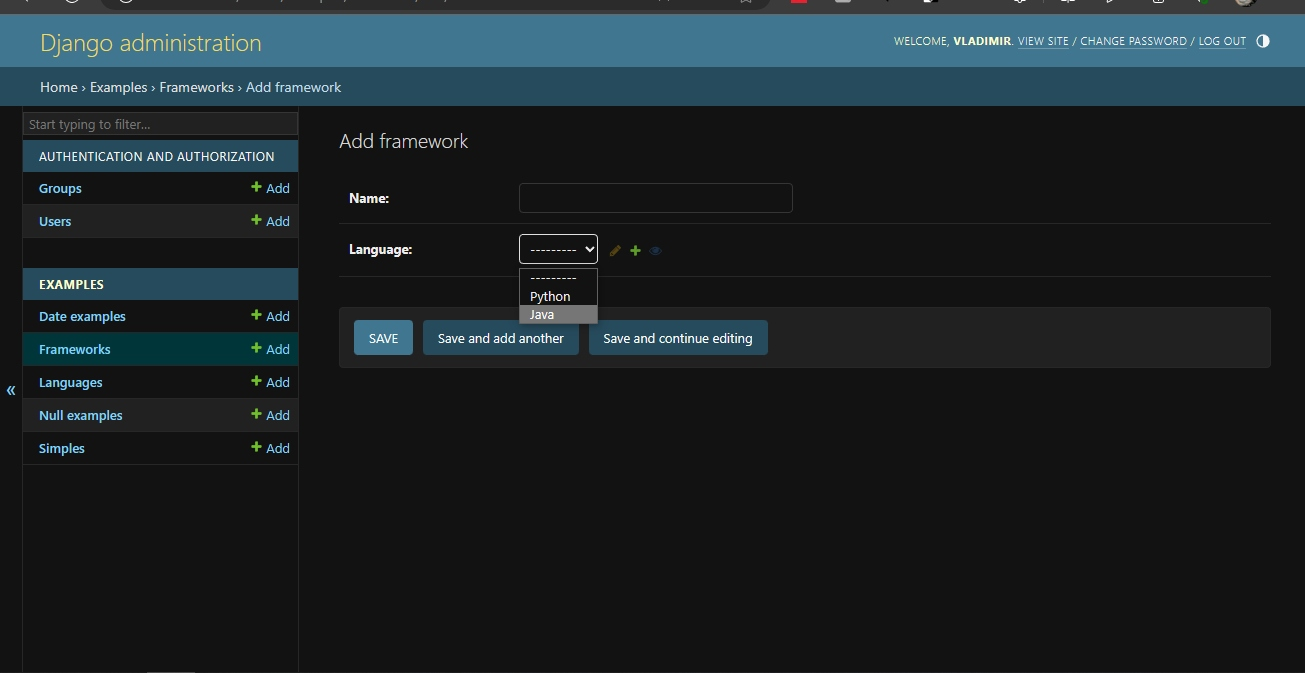
\includegraphics{img/1.jpg}
    \caption{Resultado de crear los lenguajes python y java y su vista en el modelo Framework}
    \label{fig:enter-label}
\end{figure}


\subsubsection{Query de uno a muchos}
Se añaden str a los modelos Language y Framework

\begin{lstlisting}[language=Python, caption=definir str]
class Language(models.Model):
    name = models.CharField(max_length=10)
    # Se establece que al imprimir la clase muestre name 
    def __str__(self):
        return self.name
class Framework(models.Model):
    name = models.CharField(max_length=10)
    language = models.ForeignKey(Language, on_delete=models.CASCADE)
    # Al igual que en language se usa name
    def __str__(self):
        return self.name
\end{lstlisting}

Luego al abrir el shell de python 
\begin{lstlisting}
Python 3.10.4 (tags/v3.10.4:9d38120, Mar 23 2022, 23:13:41) [MSC v.1929 64 bit (AMD64)] on win32
Type "help", "copyright", "credits" or "license" for more information.
(InteractiveConsole)
>>> from apps.examples.models import Language,Framework
>>> Framework.objects.all()   
<QuerySet [<Framework: Django>, <Framework: Flask>, <Framework: Bottle>, <Framework: Spring>]>
>>> Framework.objects.filter(language__name='Python') 
<QuerySet [<Framework: Django>, <Framework: Flask>, <Framework: Bottle>]>
>>> Framework.objects.filter(language__name='Java')   
<QuerySet [<Framework: Spring>]>
>>> Framework.objects.filter(language__name__startswith='Py') 
<QuerySet [<Framework: Django>, <Framework: Flask>, <Framework: Bottle>]>
>>> Framework.objects.filter(language__name__startswith='Pa') 
<QuerySet []>
>>> Language.objects.filter(framework__name='Spring') 
<QuerySet [<Language: Java>]>
>>> Language.objects.filter(framework__name='Bottle') 
<QuerySet [<Language: Python>]>
\end{lstlisting}

\subsection{MANY TO MANY RELATIONS}
En esta ocasion se crearan los modelos Movie y Character ya que un Character puede pertenecer a varias peliculas y una pelicula puede tener varios actores

\begin{lstlisting}[language=Python, caption=Modelos de ejemplo de ManyToManyRelations]
## Many to Many relationship example
class Movie(models.Model):
    name = models.CharField(max_length=10)

    def __str__(self):
        return self.name
class Character(models.Model):
    name = models.CharField(max_length=10)
    movies = models.ManyToManyField(Movie)
    
    def __str__(self):
        return self.name
\end{lstlisting}

Luego se procede a indagar en el shell de python

\begin{lstlisting}
Python 3.10.4 (tags/v3.10.4:9d38120, Mar 23 2022, 23:13:41) [MSC v.1929 64 bit (AMD64)] on win32
Type "help", "copyright", "credits" or "license" for more information.
(InteractiveConsole)
>>> from apps.examples.models import Movie, Character
>>> avengers = Movie(name='Avengers') 
>>> avengers.save()
>>> captain_america = Character(name='Captain America')
>>> captain_america.save()
\end{lstlisting}

Al crear captain america a diferencia de uno a muchos 
\newpage
\begin{figure}[!h]
    \centering
    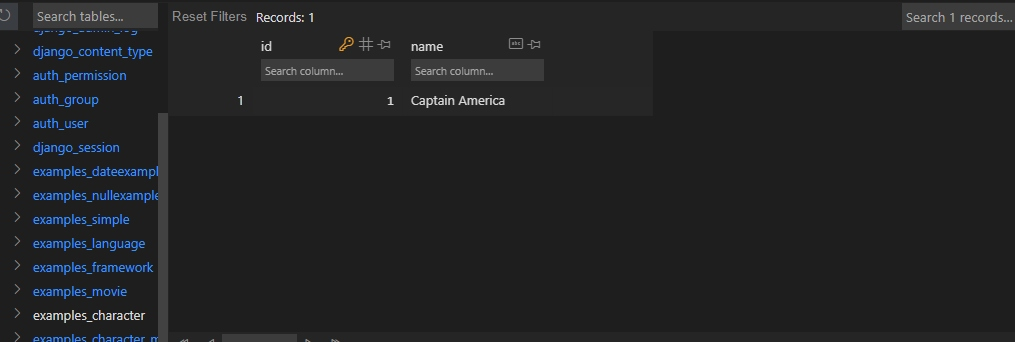
\includegraphics[scale=1.5]{img/2.jpg}
    \caption{Resultado de crear el Character captain america y su vista en la base de datos}
    \label{fig:enter-label}
\end{figure}


\begin{lstlisting}

>>> captain_america.movies.add(avengers)
>>> civil_war = Movie(name='Civil War')
>>> thor = Movie(name='Thor: The Dark World')
>>> thor_character = Character(name='Thor')
>>> civil_war.save()
>>> thor.save()
>>> thor_character.save()
>>> captain_america.movies.add(civil_war)
>>> thor_character.movies.add(avengers)
>>> thor_character.movies.add(thor)
\end{lstlisting}

Entonces al añadir las peliculas a sus respectivos actores se muestra en el admin

\begin{figure}[!h]
    \centering
    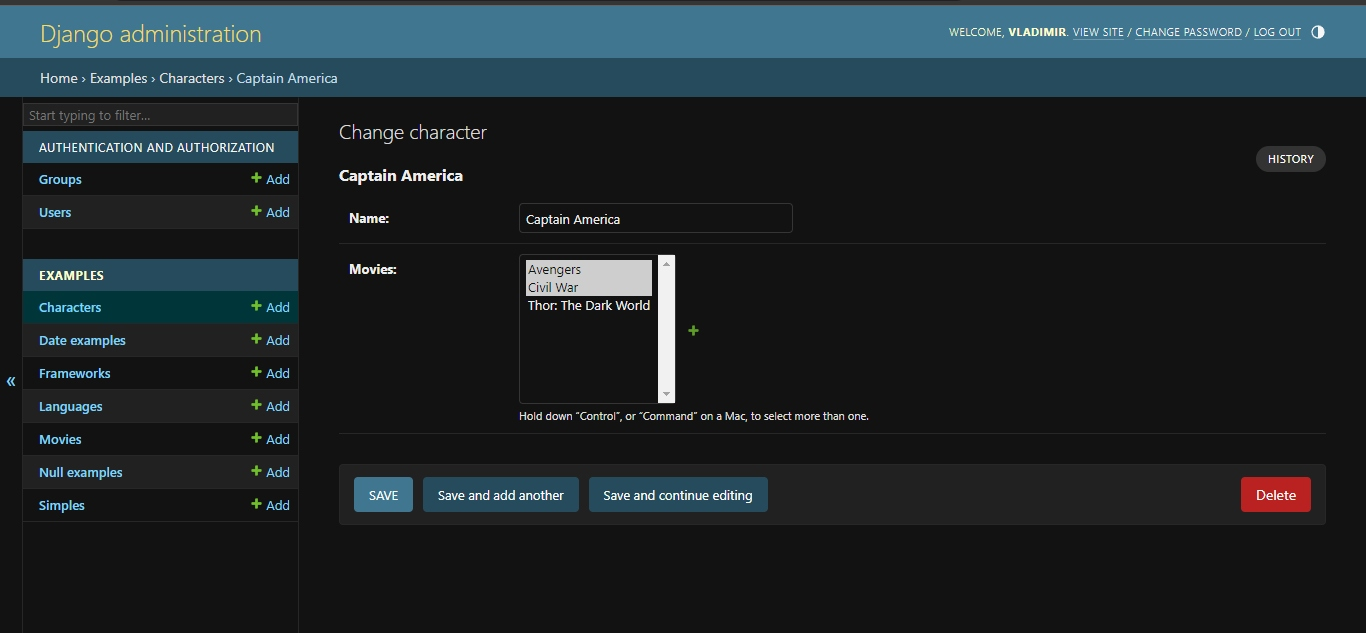
\includegraphics{img/3.jpg}
    \caption{Resultado de añadir las peliculas avengers y civil war}
    \label{fig:enter-label}
\end{figure}

\begin{figure}[!h]
    \centering
    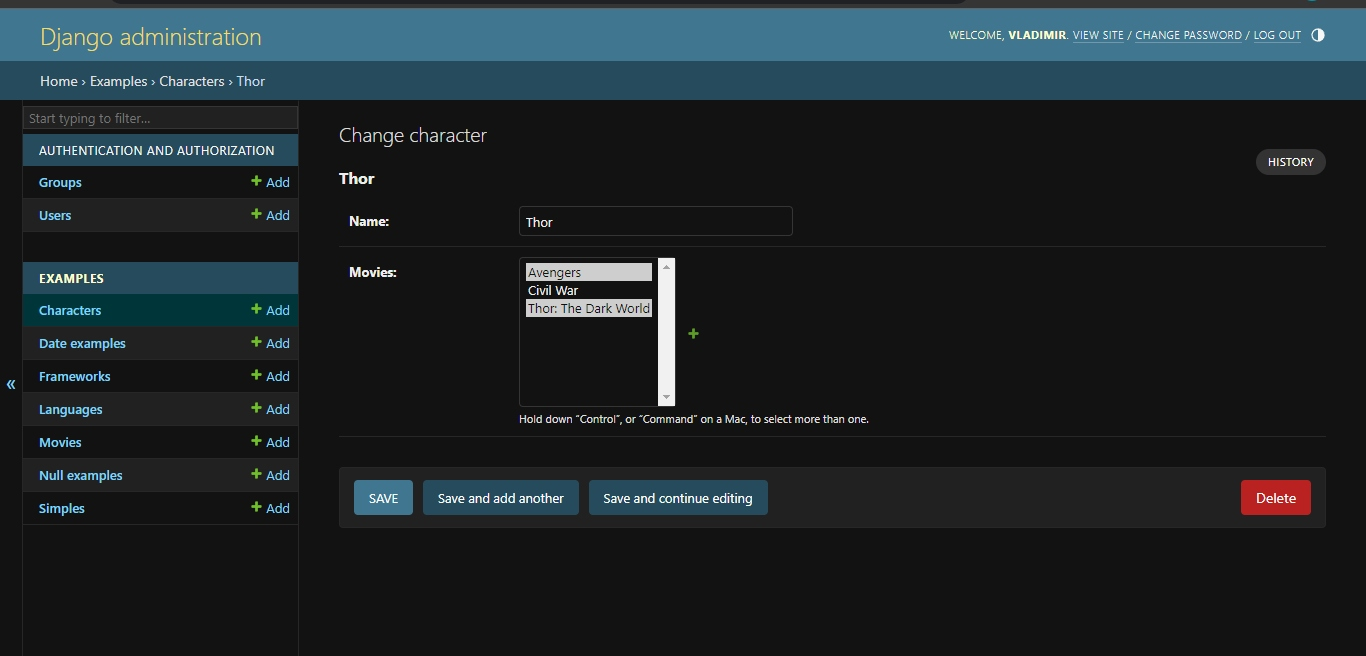
\includegraphics{img/4.jpg}
    \caption{Resultado de añadir las peliculas avengers y thor: the dark world}
    \label{fig:enter-label}
\end{figure}

\newpage

Cabe recalcar que para que la en la tabla caracter no aparece las peliculas

\begin{figure}[!h]
    \centering
    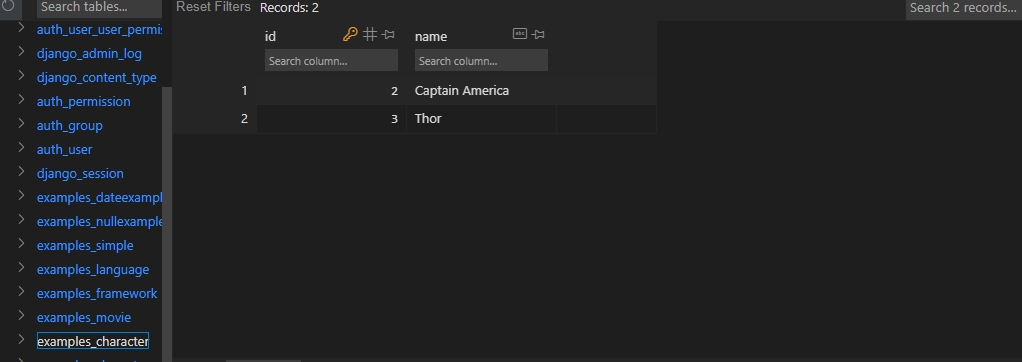
\includegraphics[scale=1.5]{img/character.jpg}
    \caption{Tabla Character}
    \label{fig:enter-label}
\end{figure}

\begin{figure}[!h]
    \centering
    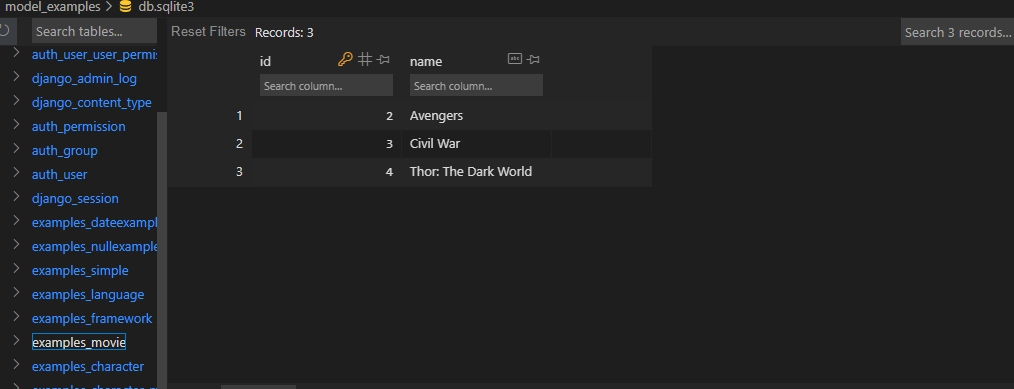
\includegraphics[scale=1.5]{img/movies.jpg}
    \caption{tabla Movies}
    \label{fig:enter-label}
\end{figure}

\newpage
Entonces con el id la tabla character y movies se conectan en otra tabla

\begin{figure}[!h]
    \centering
    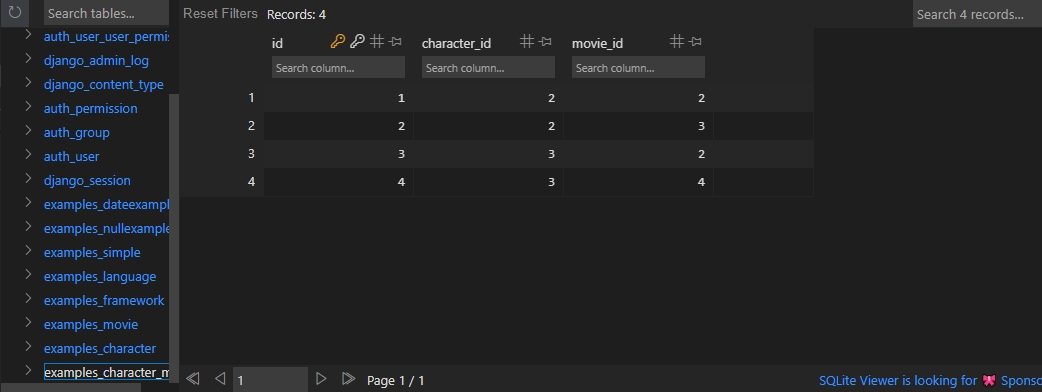
\includegraphics[scale=1.5]{img/5.jpg}
    \caption{La tabla que conecta la tabla character y movies vease los id en las tres tablas}
    \label{fig:enter-label}
\end{figure}

Tambien se puede crear nuevas peliculas usando a los Characters
\begin{lstlisting}
>>> captain_america.movies.create(name='Winter Soldier')
<Movie: Winter Soldier>
\end{lstlisting}
Y esta pelicula ya esta añadida al character captain_america

\subsubsection{Query Many To Many Relations}

\begin{lstlisting}
>>> Character.objects.filter(movies__name='Civil War') 
<QuerySet [<Character: Captain America>]>
>>> Movie.objects.filter(character__name='Captain America') 
<QuerySet [<Movie: Avengers>, <Movie: Civil War>, <Movie: Winter Soldier>]>
>>> captain_america = Character.objects.get(name='Captain America') 
>>> captain_america
<Character: Captain America>
>>> captain_america.movies.all()
<QuerySet [<Movie: Avengers>, <Movie: Civil War>, <Movie: Winter Soldier>]>
>>> avengers = Movie.objects.get(name='Avengers') 
>>> avengers
<Movie: Avengers>
>>> avengers.character_set.all()
<QuerySet [<Character: Captain America>, <Character: Thor>]>
\end{lstlisting}

\section{RENDER PDF FILE IN DJANGO}

Siguiendo las instrucciones de \cite{render_pdf_page} o \cite{video_render_pdf} 
pero con algunas modificaciones
\begin{itemize}
    \item Vamos a crear la aplicacion render_pdf
    \item el css y java script va a estar en un archivo aparte
\end{itemize}

primero como dicen el tutorial se instala por medio de pip

\begin{lstlisting}
pip install --pre xhtml2pdf 
\end{lstlisting}

Se nos instalara un monton de paquetes. \\
Luego se procede a crear la aplicacion render_pdf con todo y sus templates despues de configurar los templates en settings

\begin{lstlisting}[language=Python,caption=cambiar la configuracion de los templates]
TEMPLATES = [
    {
        'BACKEND': 'django.template.backends.django.DjangoTemplates',
        'DIRS': [os.path.join(BASE_DIR,'templates')],
        'APP_DIRS': True,
        'OPTIONS': {
            'context_processors': [
                'django.template.context_processors.debug',
                'django.template.context_processors.request',
                'django.contrib.auth.context_processors.auth',
                'django.contrib.messages.context_processors.messages',
            ],
        },
    },
]
    
\end{lstlisting}

\begin{lstlisting}[language=Python,caption=(opcional) configurar archivos static y assets]

STATIC_URL = 'static/'
STATICFILES_DIRS = [
    os.path.join(BASE_DIR, 'static')
]
STATIC_ROOT = os.path.join(BASE_DIR, 'assets')    
\end{lstlisting}

\begin{lstlisting}[caption = instalacion de render_pdf]
mkdir apps
cd apps
django-admin startapp render_pdf
\end{lstlisting}

Una vez terminado procedemos a crear un archivo llamado utils que esta en la app y tambien creamos el archivo invoice.html en templates/pdf

\begin{lstlisting}[style=ascii-tree]
model_examples/
|--- apps
       |--- examples
       |--- render_pdf
           |--- migrations
           |--- static
              |--- css
              |--- js
           |--- templates
              |--- pdf
                   |--- invoice.html
           |--- __init__.py
           |--- admin.py
           |--- apps.py
           |--- models.py
           |--- tests.py
           |--- utils.py
           |--- views.py
           
|--- model_examples
        |--- __pycache__
        |--- asgi.py
        |--- settings.py
        |--- urls.py
        |--- wsgi.py
        
\end{lstlisting}

en utils.py añadimos el siguiente codigo

\begin{lstlisting}[laguage=Python]
from io import BytesIO
from django.http import HttpResponse
from django.template.loader import get_template

from xhtml2pdf import pisa

def render_to_pdf(template_src, context_dict={}):
    template = get_template(template_src)
    html  = template.render(context_dict)
    result = BytesIO()
    pdf = pisa.pisaDocument(BytesIO(html.encode("ISO-8859-1")), result)
    if not pdf.err:
        return HttpResponse(result.getvalue(), content_type='application/pdf')
    return None
    
\end{lstlisting}

en invoide se añaden las variables invoice.id, customer_name y today para ver si imprime las variables en el pdf

\begin{lstlisting}[language=HTML]
    <body>
        <div class='wrapper'>
            <div class='header'>
                <p class='title'>Invoice {{ invoice.id }}</p>
            </div>
        <div>
        <div class='details'>
            Bill to: {{ customer_name }} <br/>
            Amount:  {{ amount }}  <br/>
            Date:  {{ today }} 
            <hr class='hrItem' />
        </div>
    </div>
    </body>
\end{lstlisting}

En views añadimos el siguiente codigo

\begin{lstlisting}[language=Python]
from django.http import HttpResponse
from django.views.generic import View
from django.template.loader import get_template
from .utils import render_to_pdf #created in step 4

class GeneratePdf(View):
    def get(self, request, *args, **kwargs):
        template = get_template('pdf/invoice.html')
        context = {
            'invoice_id': 123, 
            'customer_name': 'Vladimir Sulla',
            'amount': 12000,
            'today': "Today",
        }
        pdf = render_to_pdf('pdf/invoice.html',context)
        return HttpResponse(pdf, content_type='application/pdf')
\end{lstlisting}

finalmente en url se añade el enlace

\begin{lstlisting}[language=Python]
from django.contrib import admin
from .views import GeneratePdf
from django.urls import path

urlpatterns = [
    path('',GeneratePdf.as_view(), name="pdf"),
]
\end{lstlisting}

y en urls de projecto

\begin{lstlisting}[language=Python]
from django.contrib import admin
from django.urls import path,include

urlpatterns = [
    path('admin/', admin.site.urls),
    path('pdf/',include('apps.render_pdf.urls')),
]
\end{lstlisting}

Esta version solamente muestra el pdf. Para hacer un enlace que automaticamente descargue el pdf se añade lo siguiente

\begin{lstlisting}[language=Python,caption=funcion modificada para un enlace que descargue automaticamente]

from django.http import HttpResponse
from django.views.generic import View
from django.template.loader import get_template
from .utils import render_to_pdf #created in step 4

class GeneratePdf(View):
    def get(self, request, *args, **kwargs):
        template = get_template('pdf/invoice.html')
        context = {
            'invoice_id': 123, 
            'customer_name': 'Vladimir Sulla',
            'amount': 12000,
            'today': "Today",
        }
        pdf = render_to_pdf('pdf/invoice.html',context)
        if pdf:
            response = HttpResponse(pdf, content_type='application/pdf')
            filename = "Invoice_%s.pdf" %(12341231)
            content = "inline; filename='%s'" %(filename)
            download = request.GET.get("download")
            if download:
                content = "attachment; filename='%s'" %(filename) 
            response['Content-Disposition'] = content
            return content
        return HttpResponse('No Found')

\end{lstlisting}

\section{SENDING EMAILS IN DJANGO}
Siguiendo las instrucciones en \url{https://www.youtube.com/watch?v=X7DWErkNVJs} Creamos una pagina temporal en \url{https://temp-mail.org/}

Procedemos a crear un email temporal la pagina \url{https://temp-mail.org/}  

\begin{figure}[!h]
    \centering
    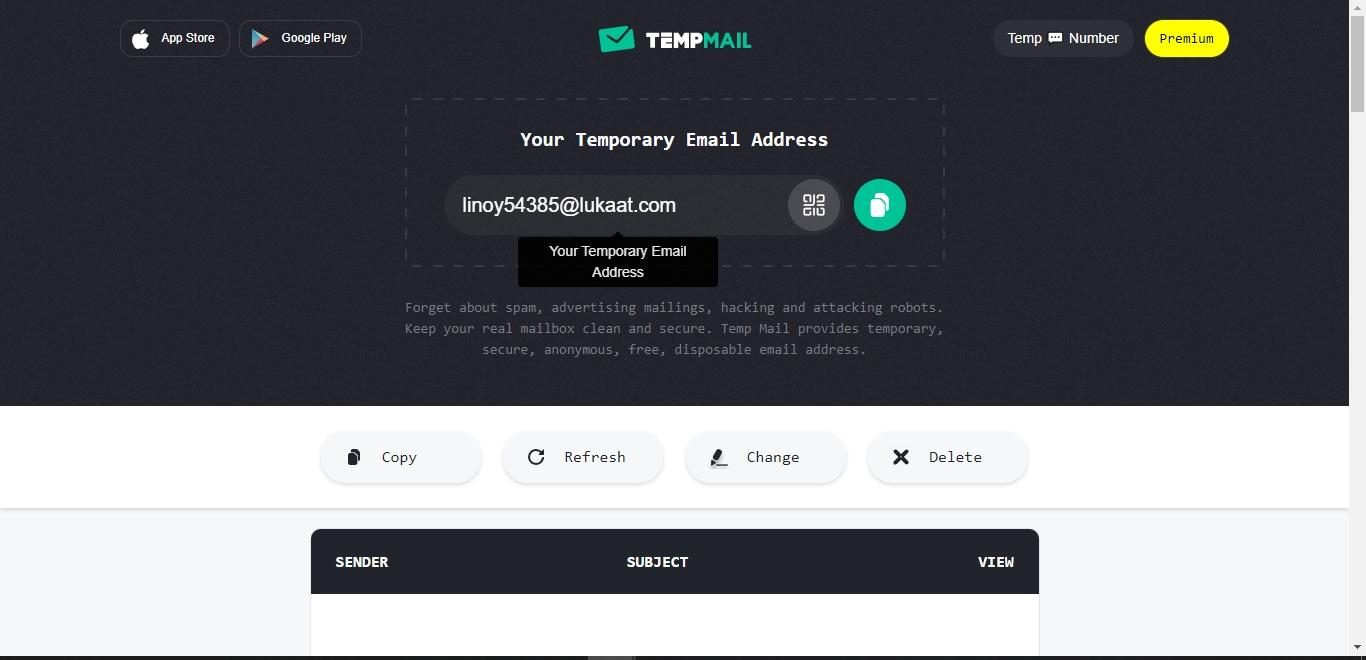
\includegraphics[scale=1.3]{img/tempemail.jpg}
    \caption{Pagina para crear un email temporal }
    \label{fig:enter-label}
\end{figure}


Luego en views creamos por el momento un metodo para ver index.html que esta en templates/send/

\begin{lstlisting}[language=Python]
from django.shortcuts import render

# Create your views here.

def index(request):
    return render(request, 'send/index.html')
\end{lstlisting}

Creamos una platilla simple en index.html

\begin{lstlisting}[language=HTML]
<!DOCTYPE html>
<html lang="en">
  <head>
    <meta charset="UTF-8">
    <meta name="viewport" content="width=device-width, initial-scale=1.0">
    <meta http-equiv="X-UA-Compatible" content="ie=edge">
    <title>HTML 5 Boilerplate</title>
    <link rel="stylesheet" href="style.css">
  </head>
  <body>
	<h1>Send a email</h1>
  </body>
</html>
\end{lstlisting}

El tutorial usa un django 2.0 que esta desactualizado pero en \cite{django_mail} esta la forma de enviar email mas actualizado

Entonces en view se cambia index por el siguiente codigo
\begin{lstlisting}[language=Python]
from django.core.mail import send_mail

send_mail(
    "Subject here",
    "Here is the message.",
    "vladimir@gmail.com",
    ["to@example.com"],
    fail_silently=False,
)
\end{lstlisting}

Finalmente dejamos la parte  mas dificil para el final, en settings.py del proyecto se procede a poner este codigo

\begin{lstlisting}[language=Python]
EMAIL_HOST = 'smtp.hushmail.com'
EMAIL_PORT = 578
EMAIL_HOST_USER = 'anthony@prettyprinted.com'
EMAIL_HOST_PASSWORD = ''
EMAIL_USE_TLS = True
EMAIL_USE_SSL = False
\end{lstlisting}

Sin embargo hushmail el cual es un software para el envio de correo es de pago y no esta disponible. De hecho se presentaron varios problemas en la autenticacion y en la forma en la que el destinatario recibia el correo sin embargo hay otra manera de hacerlo sin necesidad de crear cuenta. Cabe resaltar que esto se hizo en un SO Ubuntu dentro de una maquina virtual.

\subsection{POSTFIX}

Segun \cite{postfix} y \cite{postfixwiki} postfix es de codigo abierto y alternativa a sendmail que permite usar el localhost para envio de mails.
Entonces se procede con la instalacion

\begin{lstlisting}
sudo apt-get install postfix
\end{lstlisting}

En medio de la instalacion se nos muestra lo siguiente:

\newpage

\begin{figure}[!h]
    \centering
    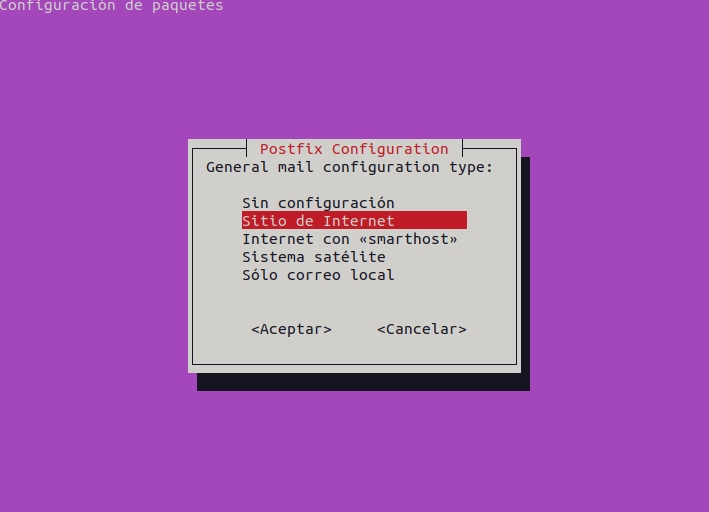
\includegraphics[scale=1.5]{img/postfix2.jpg}
    \caption{}
    \label{fig:enter-label}
\end{figure}

En donde nos indica el tipo de configuracion, Se selecciona "sitio de internet"

\begin{figure}[!h]
    \centering
    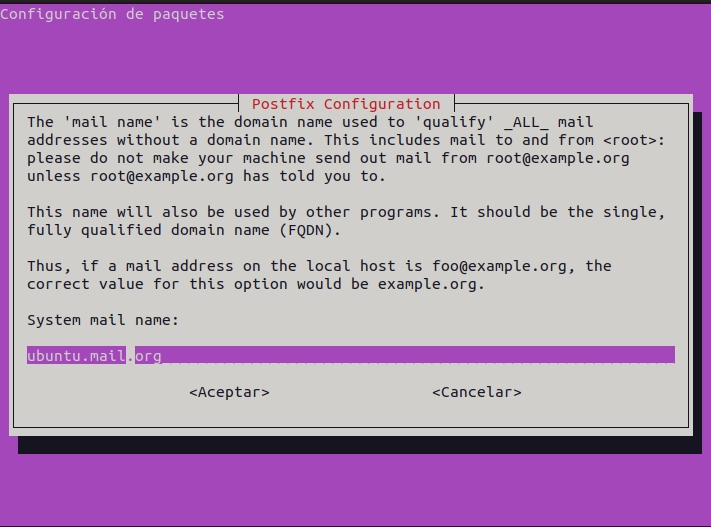
\includegraphics[scale=1.5]{img/postfix3.jpg}
    \caption{}
    \label{fig:enter-label}
\end{figure}

Luego de aceptar en la pagina anterior nos aparecera esta pantalla. Cambiamos el nombre si lo requerimos

Entoonces luego de hacer estos pasos procedemos con la configuracion en settings.py en el proyecto.

\begin{lstlisting}[language=Python]
# A partir de django 1.6+ se requiere poner esta linea de codigo 
EMAIL_BACKEND = 'django.core.mail.backends.smtp.EmailBackend'
# Como se usa postfix se pude usar el local host para enviar correo
EMAIL_HOST = 'localhost'
# El port por defecto para localhost vease la documentacion 
# de django EMAIL_PORT
EMAIL_PORT = 25
EMAIL_HOST_USER = ''
EMAIL_HOST_PASSWORD = ''
# Para evitar la authenticacion lo mas posible
EMAIL_USE_TLS = False
EMAIL_USE_SSL = False
ACCOUNT_EMAIL_VERIFICATION = 'none'
\end{lstlisting}

La informacion fue adquirida principalmente de \cite{conection_refused}

Una vez cambiado ya se puede enviar correos 

\begin{figure}[!h]
    \centering
    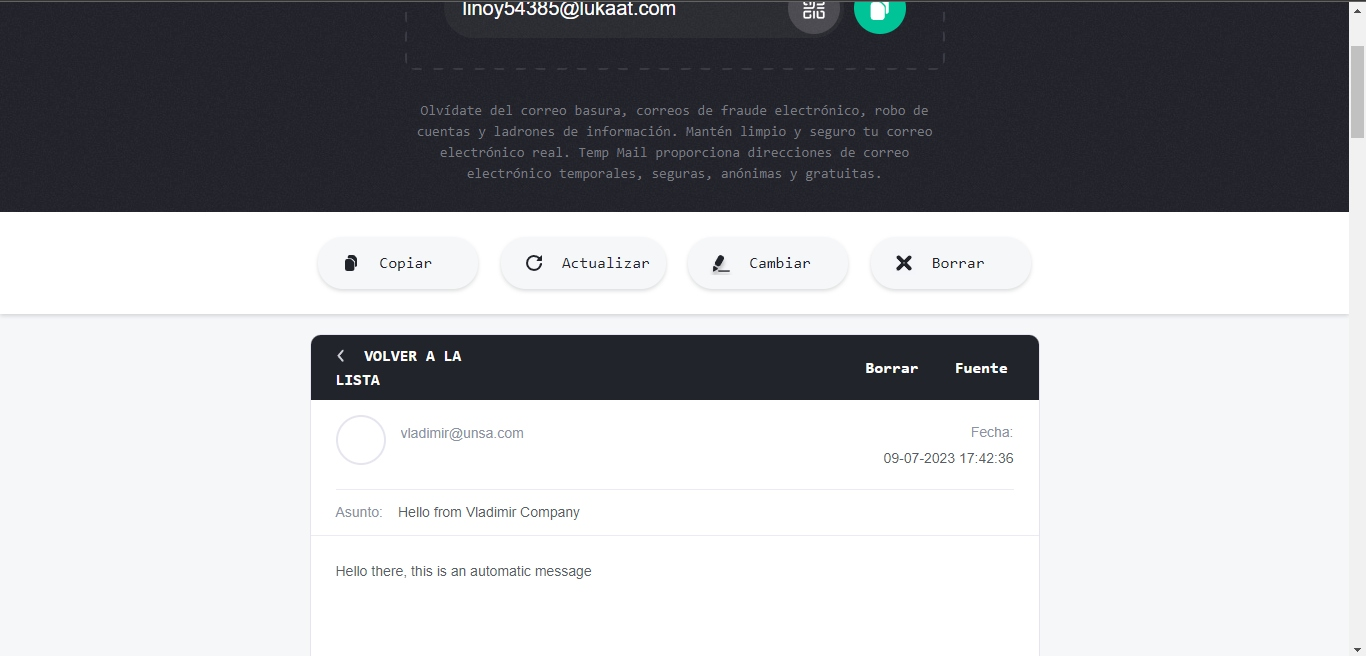
\includegraphics[scale=1]{img/TempEmailEmailGet.jpg}
    \caption{El email temporal ya puede recibir correos}
    \label{fig:enter-label}
\end{figure}

\section{COMMITS}

los ultimos commits son los siguientes:

\begin{lstlisting}
(env) $git log
commit 06ba38097adb15bca9a81f4367e86d983562ceb4 (HEAD -> main, origin/main)
Author: Vladimir Arturo Sulla Quispe <vsullaq@unsa.edu.pe>
Date:   Sun Jul 9 21:18:10 2023 -0500

    añadido comentarios a los settings de email

commit 0f48a908a3a7f7bfc5f7f9f44dd8e5a95bcd51a2
Author: alumno <alumno@ubuntu.mail.org>
Date:   Sun Jul 9 17:45:10 2023 -0500

    modificado para envio de email usando postfix

commit 2f713ef95b0bc1c3790e5e5b1f633d64c0a52e54
Author: alumno <alumno@ubuntu.mail.org>
Date:   Sun Jul 9 17:44:19 2023 -0500

    modificado el email que envia

commit 03289cf4d78fd34f0c0e3284cdbe762742b9e5e2
Author: Vladimir Arturo Sulla Quispe <vsullaq@unsa.edu.pe>
Date:   Sat Jul 8 23:14:54 2023 -0500

    añadido urls

commit c23448a302d920544a1b8c4563f540f0143bd788
Author: Vladimir Arturo Sulla Quispe <vsullaq@unsa.edu.pe>
Date:   Sat Jul 8 23:14:35 2023 -0500

    creado templates

commit 89fa641913feef1a4dbc59dd97e95927902f2f34
Author: Vladimir Arturo Sulla Quispe <vsullaq@unsa.edu.pe>
Date:   Sat Jul 8 23:14:09 2023 -0500

    añadido enalace send

commit 2dc298d8ab623626973919f7551151846e1b33c5
Author: Vladimir Arturo Sulla Quispe <vsullaq@unsa.edu.pe>
Date:   Sat Jul 8 23:13:52 2023 -0500

    tratando de que se envie correos por django

commit b8041696c4ebfbaf9c0acf820aaf35a7164108e9
Author: Vladimir Arturo Sulla Quispe <vsullaq@unsa.edu.pe>
Date:   Sat Jul 8 23:13:30 2023 -0500

    cambiado la forma en la que enviar send email

commit b179b8bcc02ab5386b1d91865e9497023fd9eacb
Author: Vladimir Arturo Sulla Quispe <vsullaq@unsa.edu.pe>
Date:   Sat Jul 8 23:12:59 2023 -0500

    cambiado nombre de apps en send

commit 9b951b4d027224a0c4a14ac9d7d89f2037507997
Author: Vladimir Arturo Sulla Quispe <vsullaq@unsa.edu.pe>
Date:   Sat Jul 8 23:12:36 2023 -0500

    cambiado conpre de apps en exampes

commit 1260f215c0774d244e477cf413a2e5931eb1283b
Author: Vladimir Arturo Sulla Quispe <vsullaq@unsa.edu.pe>
Date:   Sat Jul 8 14:16:08 2023 -0500

    registrado app en settings

commit e402f859f5e2829f09c48d9fd6e294b5add5858e
Author: Vladimir Arturo Sulla Quispe <vsullaq@unsa.edu.pe>
Date:   Sat Jul 8 14:15:42 2023 -0500

    cambiado nombre de la app send

commit d9a96f3fce768b84e6067dc30a7ab8f329c1fefc
Author: Vladimir Arturo Sulla Quispe <vsullaq@unsa.edu.pe>
Date:   Sat Jul 8 14:14:42 2023 -0500

    creada la aplicion send

commit 0d6045c3174440d101b2f3fe7fb1d7fb32d17edb
Author: Vladimir Arturo Sulla Quispe <vsullaq@unsa.edu.pe>
Date:   Sat Jul 8 13:34:44 2023 -0500

    cambiado content a response, se elimino comillas simples a la descarga de invoice

commit b45c80bd8779fa33a8f01866f303dc68c9b6b4a3
Author: Vladimir Arturo Sulla Quispe <vsullaq@unsa.edu.pe>
Date:   Sat Jul 8 13:34:08 2023 -0500

\end{lstlisting}

\printbibliography[
heading=bibintoc,
title={References}
]

\end{document}
